\section{Controbutions of the paper}
The authors of the paper rewrite visualization queries $Q$ using data reduction operator 
$M_R$ such that the visualization of the original data from query $Q$ and the visualization 
from the query $Q_R = M_R(Q)$ are similar and error free. 
\begin{figure}[h]
	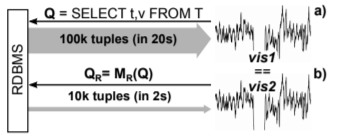
\includegraphics[width=0.5\textwidth]{qr}
	\caption{Time series visualization: a) based on original data; b) Using data reduction operator;}   
	\label{fig:1}
\end{figure}
As shown in Figure \ref{fig:1} $Q_R$ produced the same visualization as $Q$ with almost 10 times less tuples and 10 times reduced time. 
The main contributions of the paper are following:
\begin{itemize}
	\item Proposed a visualization driven query rewriting technique relying on relational operators and parameterized with width and height of the desired visualization
	\item Focusing on the detailed semantics of the line charts, they propose a visualization driven aggregation strategy that only select necessary points needed for visualization. For visualization, in every time interval which corresponds to a pixel column in the visualization they select four tuples. The starting tuple, ending tuple, max tuple and the min tuple. 
	\item 
\end{itemize}
\section{Query Rewriting}
TODO
\section{Time Series Visualization}
TODO
\section{Data Reduction Operators}
TODO
\section{Time Series Data Reduction}

